% Created 2014-12-19 Fri 14:41
\documentclass[11pt]{article}
\usepackage[utf8]{inputenc}
\usepackage[T1]{fontenc}
\usepackage{fixltx2e}
\usepackage{graphicx}
\usepackage{longtable}
\usepackage{float}
\usepackage{wrapfig}
\usepackage{rotating}
\usepackage[normalem]{ulem}
\usepackage{amsmath}
\usepackage{textcomp}
\usepackage{marvosym}
\usepackage{wasysym}
\usepackage{amssymb}
\usepackage{hyperref}
\tolerance=1000
\usepackage{fullpage}
\usepackage[backend=bibtex,sorting=none]{biblatex}
\usepackage{hyperref}
\usepackage{amsmath}
\usepackage{amssymb}
\addbibresource{telomeres.bib}
\author{Kyle M. Douglass}
\date{\today}
\title{Telomere Master Notes}
\hypersetup{
  pdfkeywords={},
  pdfsubject={},
  pdfcreator={Emacs 24.4.50.1 (Org mode 8.2.6)}}
\begin{document}

\maketitle
\tableofcontents


\section{Introduction}
\label{sec-1}
Telomeres consist of DNA tandem repeat sequences, their associated
binding proteins, and a non-coding RNA transcript. They are located at
the end of chromosomes and address two important problems in
eukaryotes: the end-replication problem and the end-protection
problem. A nice summary is provided in \cite{sfeir-jcellsci-2012}.

\subsection{Telomere composition and structure}
\label{sec-1-1}
In humans, the telomere tandem repeat sequence is TTAGGG. A telomere's
size lies between 5 and 15 kb in humans. A key feature of the telomere
end in all organisms is the 3' single-stranded G-rich overhang. In
mammals, these overhangs are 30-500 nucleotides long.

Associated with the telomeric DNA are proteins of the shelterin
complex. Shelterin is responsible for solving the end-protection problem,
though it acts in a complicated manner.


The six known shelterin proteins are TRF1, TRF2, RAP1, TIN2, TPP1, and
POT1. TRF1 and TRF2 bind to the duplex region of the DNA; POT1 coats
the overhang with oligonucleotide/oligosaccharide binding folds. TIN2
has a bridging function since it interacts simultaneously with TRF1,
TRF2, and TPP1.

In addition to the shelterin proteins, there are telomere-associated
proteins that are recruited by shelterin to act as ``accessory
factors.''

The long non-coding RNA might be important for telomere maintenance
and function, though little is known about the underlying molecular
mechanisms.

\subsection{Telomeres and the end-replication problem}
\label{sec-1-2}
The telomerase enzyme solves the end-replication problem and helps
counteract telomere erosion. The mechanisms underlying telomere length
regulation in mammlian cells are not fully understood, though some key
factors are known.

For example, overexpressing TRF1 in cancer-derived human cells leads
to telomere shortening, whereas depleting telomeres of TRF1 results in
elongation. Reducing levels of TRF2 and TIN2 leads to telomere
extension. There are also repressive histone marks on telomeric
chromatin. Deletion of these marks correlates with large elongations
of telomeres.

\subsection{Mammalian telomeres have nucleosomes}
\label{sec-1-3}
Mammalian telomeres are enriched with repressive histone marks,
including H3K9me3 and H4K20me3 and the heterochromatin-specific
factors chromobox homolog (CBX) 1, 3, and 5. Depleting these marks
correlates with telomere elongation.

\section{Shelterin and its role in telomere functioning}
\label{sec-2}
\begin{itemize}
\item Do the shelterin proteins always come in a complete unit, or do the
ratios of the amounts of the various shelterin proteins vary from
telomere to telomere?
\item Do the increased sizes in TRF1 correspond to telomeres having longer
genomic lengths?
\end{itemize}

\subsection{TRF1 controls human telomere lengths}
\label{sec-2-1}
TRF1 was found to control the length of human telomeres
\cite{vansteensel-nature-1997}. The authors both overexpressed TRF1
and reducing the binding of TRF1 to telomeres and observed a gradual
shortening and lengthening of telomeres. The expression of telomerase
was not changed, which suggested that TRF1 somehow inhibits the action
of telomerase.

\subsection{TRF2 is linked to the DNA repair machinery}
\label{sec-2-2}
Deleting TRF2 results in the activation of the kinase ATM and triggers
the accumulation of DNA damage factors, including H2AX and 53BP1
\cite{sfeir-jcellsci-2012}. Furthermore, in the absence of TRF2,
ligase 4- and Ku-mediated NHEJ repair is activated at telomeres, which
results in chromosome end-to-end fusions \cite{sfeir-jcellsci-2012}.

\section{Polymer simulation and chromatin modeling}
\label{sec-3}
Polymer simulations are now becoming useful tools for modeling
experimental data on chromatin and predicting other structural
features of DNA \cite{rivetti-jmolbiol-1996, giorgetti-cell-2014}.

Within the context of this telomere project, we wanted to simulate a
particular chromatin model, the wormlike chain, and compare it to the
measured telomere sizes. This would allow us to estimate what
combination of values for the model parameters, the chain's contour
length and its persistence length, was most likely to have produced
our data.

\subsection{Introduction to the polymer models}
\label{sec-3-1}
Polymers are molecular and macromolecular chains that are found
throughout both the natural and the man-made world. Because of their
ubiquity, tools for studying their properties find great utility in
the physical and life sciences.

The study of polymer physics involves coping with complexity. Many
polymers are comprised of a very large number of subunits. For
example, DNA is a polymer that consists of a linear chain of tens of
millions of nucleic acids. Because of the large number of molecular
degrees of freedom, statistical mechanics and computer simulations are
the basic tools for understanding polymer structure.

This work focuses on the computer simulation of one important polymer
model, the wormlike chain (WLC). It was originally developed by Kratky
and Porod to incorporate the flexibility of a polymer into the models
of the time \cite{kratkyporod-1949}. This flexibility emerges from the
underlying details of the electronic bonds that hold the atoms and
molecules in the chain together. Despite the fact that it is now over
65 years old, the WLC still finds many uses in describing physical
phenomena. Furthermore, its details are still being uncovered by
scientists.

This work first describes the basic theory. After this, the algorithm
used to generate the 3D chains is explained. It is one of the simpler
algorithms and produces the essential results of the model. Finally, I
describe how the algorithm is implemented on the computer, using
Python as a programming language.

\subsection{Theory of the wormlike chain}
\label{sec-3-2}
In the simplest WLC model, we treat the polymer as a semiflexible and
homogeneous rod with a negligible thickness and a length $L_c$, known
as the contour length. The flexibility of the rod is described by its
persistence length $\ell_p$. Intuitively, the persistence length is
the average length over which the polymer remains approximately
straight. Polymers with a longer persistence length will be more rigid
than shorter ones.

Mathematically, the persistence length is the characteristic length
describing the exponential decay of the tanget-tanget correlation
function \cite{phillips-pbotc-2009},


\begin{equation}
  \label{eq-tantancorr}
  \left< \mathbf{t} \left( s \right) \cdot \mathbf{t} \left( 0 \right) \right> \sim \exp \left( s / \ell_p \right)
\end{equation}

where $\mathbf{t} \left( s \right)$ is the unit vector tangent to the
polymer at the one-dimensional coordinate $s$ along the polymer. For
distances $s$ much greater than $\ell_p$, \eqref{eq-tantancorr}
states that there will be no correlation in the direction that the
tangent vectors point.

The subunits that make up most polymers are very small molecules and
are thus subject to agitation by the random collisions with other
molecules in their environment. This is especially pertinent to
polymers in aqueous environments, where collisions with the solvent
molecules cause the polymer to change shape and conformation many
times a second. According to Boltzmann's statistics, the probability
that a semiflexible polymer in thermodynamic equilibrium will be found
in one of any of its possible conformations at an instant in time is
proportional to the Boltzmann factor

\begin{equation}
  P \left( U \right) \sim \exp \left( -\frac{U}{k_B T}\right)
\end{equation}

where $P \left( U \right)$ represents of the probability of observing
a polymer conformation with associated internal energy $U$, $k_B$ is
Boltzmann's constant and $T$ is the temperature of the system. The
fact that it takes energy to bend the polymer into a particular
conformation reflects the ``semiflexible'' qualities of the polymer.

The energy $U$ required from the environment to achieve a given
conformation can be determined by dividing the polymer into many short
sections such that it can be reprensented as the summation of the
energies of many small circular arcs. The energy required to bend a
rod with Young's modulus $E$, moment of 

\subsection{Simulation Testing}
\label{sec-3-3}

\subsubsection{Accuracy as a function of segment length and number of chains}
\label{sec-3-3-1}
The purpose of the simulations is to compute the probability
distribution function for randomly selecting a telomere with a certain
radius of gyration from a population of telomeres. This requires that
a large number of conformations to be generated so that the
distribution function is accurate. First, we must know how many
conformations and are required and the size of the individual segments
to accurately reflect the mean radius of gyration of the corresponding
theoretical polymer.

In the simulation, the polymer is constructed from a number of
equal-sized segments. (The last segment can be shorter than all the
others if a non-integer value is supplied as a parameter for the
polymer contour length.) In addition, the Path object and its children
in the simulation code treat all distances in segment units, i.e. a
distance of 1 represents 1 segment.

The agreement of the mean radius of gyration from the simulation and
the theoretical expression for the radius of gyration is a function of
this segment length. Intuitively, the segment length must be short
enough to accurately model the conformations of the polymer; if it's
too large, the accuracy of the mean $R_g$ values can be so large that
we cannot expect that the probability distribution of $R_g$ values to
reflect the model.

Fig. \ref{fig-accuracy1} displays the errors between the simulated
mean radius of gyration and the theoretical one using version 0.1 of
the code. The polymer chains were 25,000 bp long. Values for the
linear packing density and the persistence length were taken from the
range $\left[ 10, 30, 50, 70, 90 \right]$ and $\left[ 10, 30, 50,
\ldots, 170, 190\right]$, respectively. For each pair of these values,
1000 polymer confirmations were simluated and their mean $R_g$
calculated from the discretized probability distribution generated by
the simulation. Importantly, the segment length in user-defined units
was 0.4 nm, or 25 times smaller than the smallest persistence
length. The highest error is $0.05\%$. Note that errors are defined by
the absolute difference between simulated and theoretical $R_g$,
divided by the theoretical value for $R_g$.

\begin{figure}[htb]
\centering
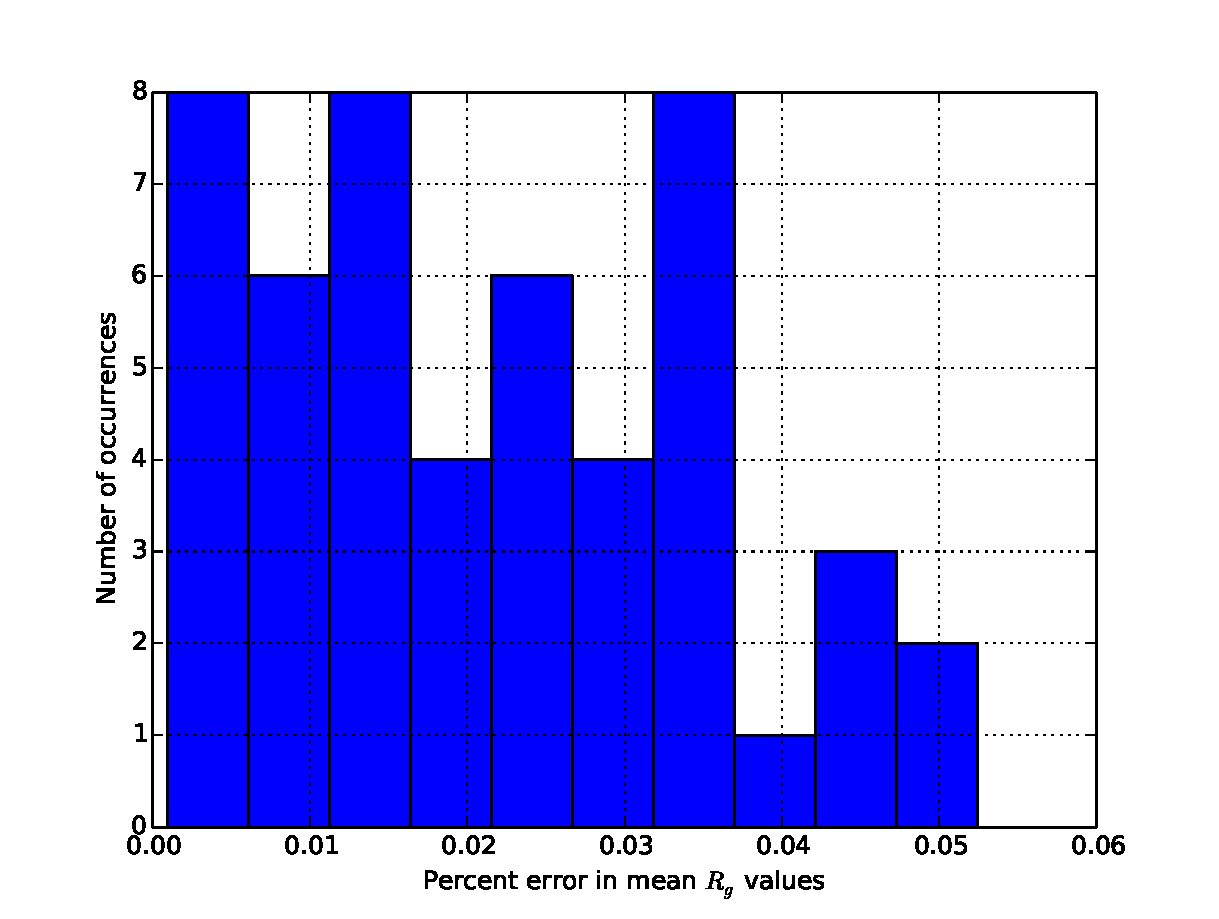
\includegraphics[width=.9\linewidth]{./images/accuracy1.pdf}
\caption{\label{fig-accuracy1}The accuracy of the mean radii of gyration for a number of polymer experiments with different packing densities and persistence lengths. 1000 polymer conformations were simulated for each parameter pair. Each segment was 0.4 nm long. The code version is 0.1.}
\end{figure}

In \ref{fig-accuracy2}, the errors are displayed for the same
simulation as above, but with a segment length equal 1 nm, or 10 times
smaller than the smallest persistence length tested. The errors appear
roughly the same, which suggests that a segment length on the order of
1 nm is a good length for accurate simulation of chromatin polymers in
these range of parameters.

\begin{figure}[htb]
\centering
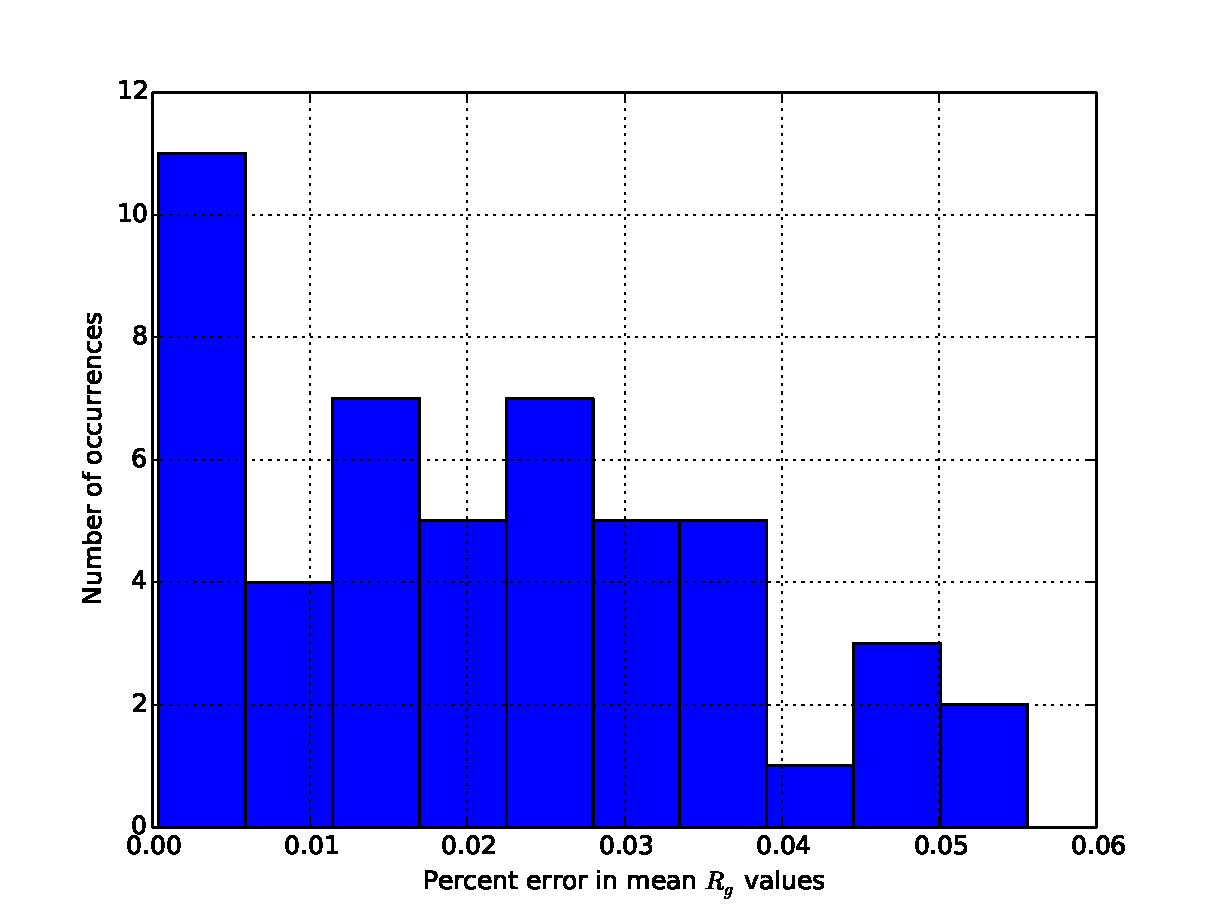
\includegraphics[width=.9\linewidth]{./images/accuracy2.pdf}
\caption{\label{fig-accuracy2}Errors between simulation and theory for the same simulation as parameters as in the previous graph, but with a segment length of 1 nm.}
\end{figure}

Finally, in \ref{fig-accuracy3} the errors are displayed for a
simulation with the same range of values for packing density and
persistence length, a segment length of 0.4 nm (25 times less than the
smallest persistence length tested, and only 100 polymers simulated
for each pair of values. Note that range of errors is about three
times as high as when 1000 polymers were tested.

\begin{figure}[htb]
\centering
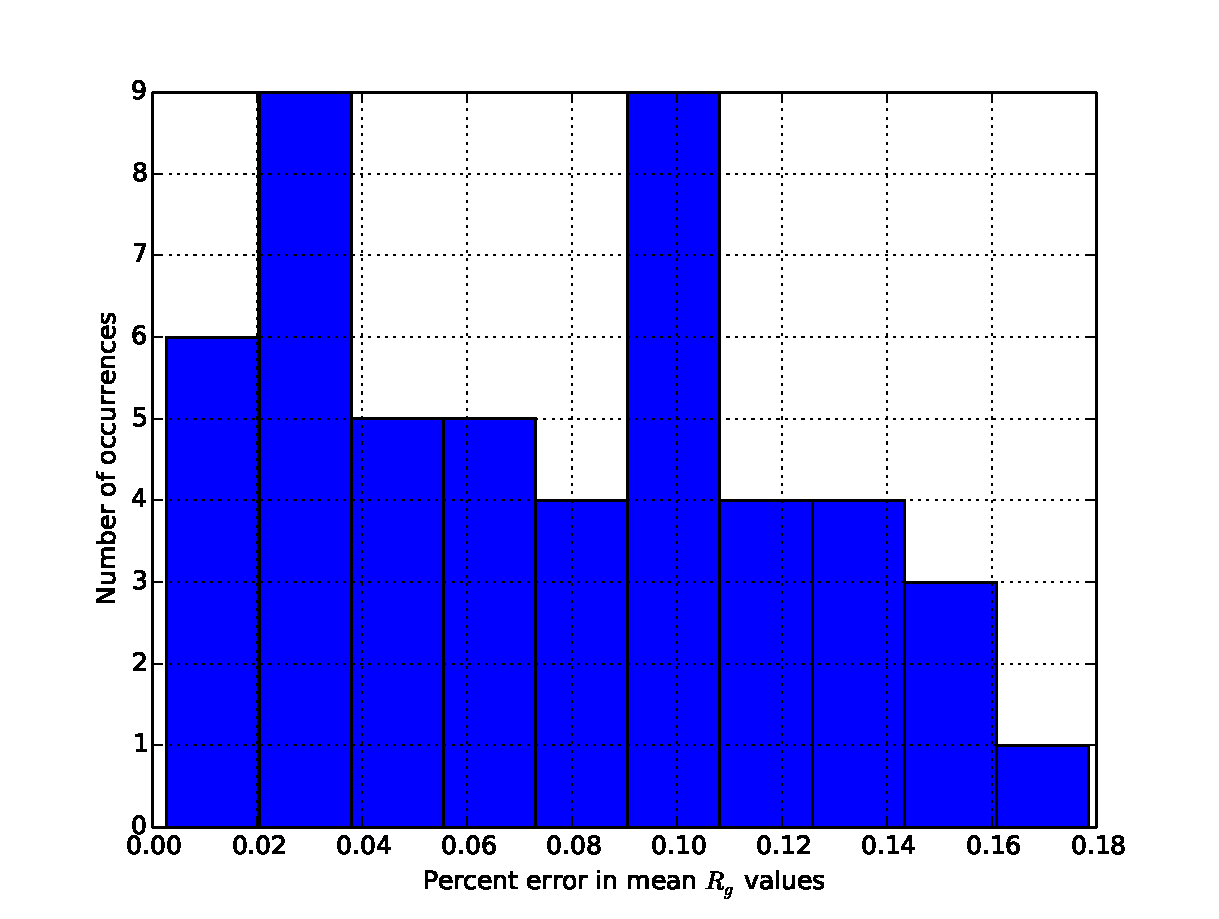
\includegraphics[width=.9\linewidth]{./images/accuracy3.pdf}
\caption{\label{fig-accuracy3}Errors for a simulation with 100 polymer conformations and 0.4 nm length segments.}
\end{figure}

These results suggest that a segment length of 0.1 nm and a minimum of
1000 bp be used to create the probability distribution function for a
chromatin polymer of a single contour length (25000 bp in these
examples). When the population also involves sampling multiple contour
lengths, more polymers will likely be required.

\subsubsection{Problems with saving histograms in the database}
\label{sec-3-3-2}
\textit{<2014-12-19 Fri>}
In version 0.1 and 0.2 of the code, the results of the radii of
gyration are saved as histograms with the bin size determined by
the method in Ref. \cite{scott-biometrika-1979}. This format
however creates a problem when performing the maximum likelihood
estimation on the polymer model parameters.

The problem lies in the tails of the distribution. In the tails, a
few bins in the histograms of the simulated gyration radii may be
empty, meaning the probability of measuring a telomere with $R_g$
value in that range is zero. However, some of the data may
actually fall into that bin, so the \textbf{log}-likelihood of seeing
that data is minus infinity.

A temporary workaround is to catch the divide-by-zero warnings
that Python throws when the numpy log function returns -inf and
instead assign the bin a probability of a very small number. This
is not satisfactory, though since the relative log-likelihoods for
different parameter pairs may be incorrectly weighted according to
how many datapoints fall within these zero-probability bins.

A better solution is to try estimating a continuous probability
density function from the simulated $R_g$ data. One way to do this
is a technique called kernel density estimation, where each point
is assigned a kernal function of equal weight and varying
size. Each function is then summed to produce a smooth, continuous
pdf of the discrete data.

\subsubsection{Timing}
\label{sec-3-3-3}
In version 0.2 of the code, I rewrote the main loop for creating
the 3D wormlike chains. After profiling the Python code, I
concluded that this rewrite sped it up by a factor of four. Most
of the rewrite came from continuously normalizing a new
displacement vector with numpy's norm() function during each
iteration of the loop. I instead made this inline and directly
called the Fortran function nrm2. In addition, I made the cross
product operation inline as well in pure Python.

I also timed a simulation with the following parameters: $c =
    \left[10, 30, \ldots , 90\right]$, $\ell_p = \left[ 10, 30,
    \ldots, 190 \right]$, and 10 chains for each pair of values
$\left(c, \ell_p\right)$.  This took approximately 30 seconds.

Simulating 50,000 chains with the same set of parameter pairs
should take 150,000 seconds according to this estimation. I
performed the simulation with the version 0.2 code and found the
actual time to be about 156,900 seconds, which is not far off the
estimation.
\subsubsection{Tests to be performed}
\label{sec-3-3-4}
These are the crucial tests to be performed on the polymer simulation
code before simulating polymer conformations.

\begin{enumerate}
\item $\boxtimes$ The dependence of the simulated mean RG on segment length.
This test was performed with code version 0.1 on \textit{<2014-11-28 Fri>}.
\item $\boxtimes$ The dependence of the simulated mean RG on the number of
paths. Test performed with code version 0.1 on \textit{<2014-11-28 Fri>}
\end{enumerate}

\printbibliography
% Emacs 24.4.50.1 (Org mode 8.2.6)
\end{document}
